\documentclass{../../../fal_assignment}
\graphicspath{ {../../../} }

\usepackage{amsmath}
\usepackage{enumitem}
\setlist{nosep} % Make enumerate / itemize lists more closely spaced
\usepackage[T1]{fontenc} % http://tex.stackexchange.com/a/17858
\usepackage{url}
\usepackage{todonotes}

\usepackage{listings}
\lstset{
	basicstyle=\ttfamily,
	frame=single,
	showstringspaces=false,
	breaklines=false,
	prebreak={\space\hbox{\textcolor{gray}{$\hookleftarrow$}}}
}
\lstset{
	commentstyle=\ttfamily\textit,
	keywordstyle=\ttfamily\textbf,
	stringstyle=\ttfamily,
	rulecolor=\color{black}
}
\lstset{language=C++}

\newcommand{\colvec}[2]{\begin{pmatrix}#1\\#2\end{pmatrix}}
\newcommand{\colxy}[1]{\colvec{x_{#1}}{y_{#1}}}

\title{Worksheet A}
\author{Dr Ed Powley}
\module{COMP270}
\version{1.0}

\begin{document}

\maketitle

\section*{Introduction}

In this worksheet you will use cubic B\'ezier curves to implement a top-down 2D race track.

Begin by \textbf{forking} the following git repository:

\begin{center}
	\url{https://github.com/Falmouth-Games-Academy/comp270-worksheet-A}
\end{center}

\textbf{Complete} the tasks described below, remembering to \textbf{commit} your work regularly.
To submit your work, open a \textbf{pull request} from your forked repository to the original repository.

The template program in this repository has a number of empty functions which the tasks below ask you to fill in. Feel free to add or modify any other code that makes your solutions easier to write or maintain ---
for example you are encouraged to add your own helper methods to the provided classes in order to enable code reuse.

The following video demonstrates what successfully completed solutions to the tasks should look like:

\begin{center}
	\url{https://youtu.be/KugZcz6YZTQ}
\end{center}

\section*{Background}

Given four points in 2D space
$$ \mathbf{p}_0 = \colxy0, \mathbf{p}_1 = \colxy1, \mathbf{p}_2 = \colxy2, \mathbf{p}_3 = \colxy3 \,, $$
a \emph{cubic B\'ezier curve} is defined by
$$ b(t) = (1-t)^3 \mathbf{p}_0 + 3(1-t)^2t \mathbf{p}_1 + 3(1-t)t^2 \mathbf{p}_2 + t^3 \mathbf{p}_3 $$
where $0 \leq t \leq 1$. See Figure~\ref{fig:bezier}.

\begin{figure}[ht]
	\begin{center}
		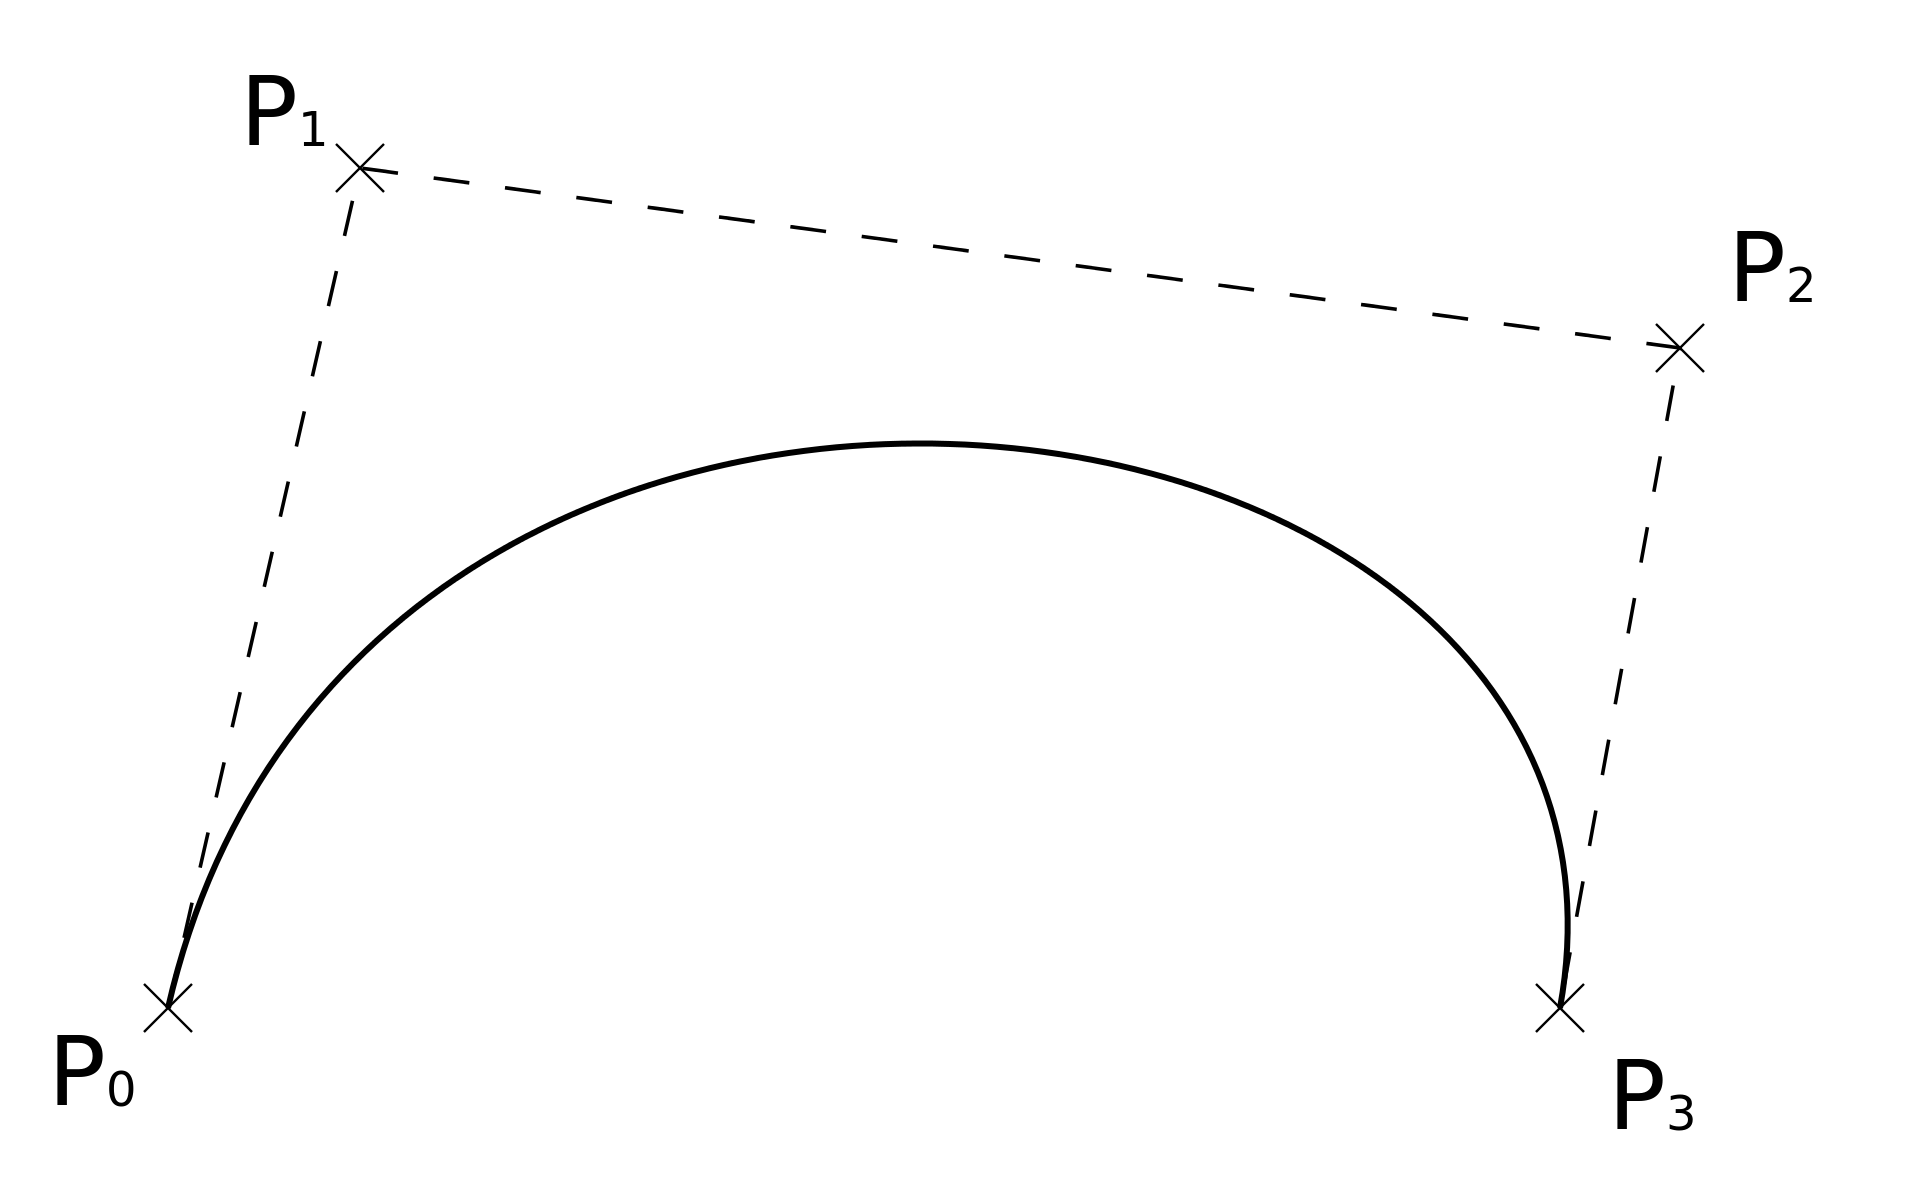
\includegraphics[width=0.6\textwidth]{bezier}
	\end{center}
	\caption{A cubic B\'ezier curve. Image source: \protect\url{https://commons.wikimedia.org/wiki/File:Bezier_curve.svg}.}
	\label{fig:bezier}
\end{figure}

The provided template program defines a \lstinline{Bezier} class which represents a cubic B\'ezier curve.
The program also defines a race track as a chain of B\'ezier curves,
stored as \lstinline{std::vector<Bezier> m_track}.
The curves are set up such that the end point of one equals the start point of the next, and the start point of the first equals the end point of the last, giving the appearance of a continuous loop.

\section*{Task 1: drawing B\'ezier curves}

For the purposes of rendering, a B\'ezier curve can be approximated by a series of straight lines.
If $b(t)$ denotes the point on the curve with parameter $t$,
then the curve can be drawn as a sequence of $n$ line segments by drawing lines between points
$$ b\left(\frac{i}{n}\right) \text{ and } b\left(\frac{i+1}{n}\right) $$
for $i = 0, \dots, n-1$. For example if $n=2$, the curve is approximated by two lines: one from $b(0.0)$ to $b(0.5)$, and one from $b(0.5)$ to $b(1.0)$. The larger $n$ is, the smoother the curve appears.

In the code, the \lstinline{Bezier} class has a \lstinline{draw} method which currently does nothing.
\textbf{Implement} the method so that it draws the curve, using \lstinline{SDL_RenderDrawLine} or \lstinline{SDL_RenderDrawLineF} to draw the line segments. The number of segments ($n$ in the above discussion) should be defined as a constant so that it can be tuned; a value of $20$ is a good default.

\section*{Task 2: following the curve}

If the track is made up of $n$ curves, denoted $b_0, \dots, b_{n-1}$, then we can represent a position
along the track as a number $s$ with $0 \leq s \leq n$.
The integer part of $s$ gives the curve number, and the fractional part gives the $t$ parameter along the curve. For example, $s=1.2$ represents curve $1$ and parameter value $0.2$, so $b_1(0.2)$.

In C++, the integer part of a floating point number can be found\footnote{Some caution is required using these with negative numbers; however we always have $s \geq 0$ so this is not an issue here.} by using \lstinline{static_cast<int>(s)}.
The fractional part can be found using \lstinline{fmodf(s, 1.0f)}.

The \lstinline{Application} class has a \lstinline{drawCarOnTrack} method which currently does nothing.
It takes a single argument, \lstinline{position}, which acts as $s$ in the discussion above.
\textbf{Implement} the method so that it draws a car sprite at the given position on the track;
when done correctly, the sprite will be animated performing laps of the track.

Your implementation should call \lstinline{drawCar} to actually draw the sprite.
This function takes two arguments: a position (as a \lstinline{Vector2}), and an angle.
Pass an angle of 0 for now; the next task is to calculate a more appropriate angle.

\section*{Task 3: facing the tangent}

At a point with parameter $t$, the tangent to the cubic B\'ezier curve is given by\footnote{Those of you who know calculus can verify that this is the derivative of $b(t)$ with respect to $t$.}
$$ b'(t) = 3(1-t)^2(\mathbf{p}_1 - \mathbf{p}_0) + 6(1-t)t(\mathbf{p}_2 - \mathbf{p}_1) + 3t^2 (\mathbf{p}_3 - \mathbf{p}_2) \,. $$

\textbf{Modify} your implementation of \lstinline{Application::drawCarOnTrack} such that the car is drawn
facing along the tangent to the curve --- that is, in the direction of the track.
Modify the angle passed to \lstinline{drawCar} to achieve this.
You will find the \lstinline{atan2f} function useful in converting from the tangent vector to the required
angle; however note that \lstinline{atan2f} returns an angle in radians whereas \lstinline{drawCar}
expects an angle in degrees.

\section*{Task 4: movement speed}

You will notice that the car appears to speed up and slow down on certain parts of the track.
This is because we are incrementing $t$ by a constant amount every frame (in \lstinline{Application::updateCarPosition}, but this does not necessarily
correspond to a constant distance along the curve.

\textbf{Modify} the implementation of \lstinline{Application::updateCarPosition} to achieve a more consistent movement speed.
Figuring out exactly how to achieve this is part of the exercise.

\begin{markingrubric}
	\firstcriterion{Basic competency threshold}{40\%}
		\grade\fail	A reasonable attempt at the worksheet was not submitted by the formative deadline.
	\gradespan{5}{A reasonable attempt at the worksheet was submitted by the formative deadline.
		\par		There is no evidence of academic misconduct.}
		
    \criterion{Functional coherence}{40\%}
        \grade\fail None of the tasks have been attempted.
		\grade Task 1 has been attempted and partially completed.
		\grade Task 1 has been successfully completed.
		\grade Tasks 1 and 2 have been successfully completed.
		\grade Tasks 1--3 have been successfully completed.
		\grade Tasks 1--4 have been successfully completed.

    \criterion{Maintainability}{20\%}
        \grade \fail The code is only sporadically commented, if at all, or comments are unclear.
            \par Few identifier names are clear or inappropriate.
            \par Code formatting hinders readability.
        \grade The code is well commented.
            \par Some identifier names are descriptive and appropriate.
            \par An attempt has been made to adhere to a consistent formatting style.
             \par There is little obvious duplication of code or of literal values.           
        \grade The code is reasonably well commented.
            \par Most identifier names are descriptive and appropriate.
            \par Most code adheres to a sensible formatting style.
             \par There is almost no obvious duplication of code or of literal values.   
        \grade The code is reasonably well commented, with appropriate high-level documentation.
            \par Almost all identifier names are descriptive and appropriate.
            \par Almost all code adheres to a sensible formatting style.
             \par There is no obvious duplication of code or of literal values. Some literal values can be easily ``tinkered''. 
        \grade The code is very well commented, with comprehensive appropriate high-level documentation.
            \par All identifier names are descriptive and appropriate.
            \par All code adheres to a sensible formatting style.
             \par There is no obvious duplication of code or of literal values. Most literal values are, where appropriate, easily ``tinkered''.  
        \grade The code is commented extremely well, with comprehensive appropriate high-level documentation.
            \par All identifier names are descriptive and appropriate.
            \par All code adheres to a sensible formatting style.
            \par There is no duplication of code or of literal values. Nearly all literal values are, where appropriate, easily ``tinkered''.  
\end{markingrubric}

\end{document}
